
\documentclass{beamer}


\usetheme{Warsaw}
\usecolortheme{crane}


\title{Fourier Series Fundamentals}
\subtitle{Mathematical Methods in the Physical Sciences}
\author{Steve Mazza}
\institute[Naval Postgraduate School]
{ 
    Naval Postgraduate School \\
    Monterey, CA \\
    
\includegraphics[height=3cm]{images/NPS_logo.jpg}
}
\date {SE3030, Winter/2014 \\ Quantitative Methods of Systems Engineering}
\subject{Quantitative Methods of Systems Engineering}


\begin{document}

\frame{\titlepage}


\frame{{Introduction}
    Fourier series are like power series but are only used to represent periodic functions.
    \begin{center}
        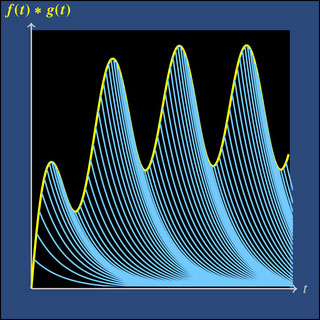
\includegraphics[scale=0.4]{images/fourier.jpg}
    \end{center}
}


\frame{{Periodic Functions}
    \begin{block}{Simple Harmonic Motion}
        An object executing simple harmonic motion if its displacement from equilibrium can be written as $A \text{ sin } \omega t$ or $A \text{ cos }\omega t$ or $A\text{ sin }\left( \omega t+\phi \right)$.
    \end{block}
    \begin{center}
        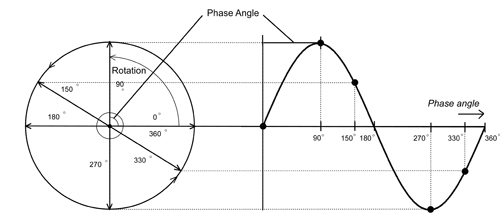
\includegraphics[height=4cm]{images/simple-harmonic-motion.jpg}
    \end{center}
}


\frame{{Periodic Functions (continued)}
    The $x$ and $y$ components are $\left( A\text{ cos }\omega t, A\text{ sin }\omega t \right)$.  In the complex plane this could be rewritten as
    \begin{align*}
        z &= x+iy \\
        &= A\left( \cos\omega t+i\sin\omega t \right) \\
        &= Ae^{i\omega t}
    \end{align*}

    The \emph{amplitude} is the maximum displacement from equilibrium and the \emph{period} is the time of one complete oscillation.
}


\frame{{Applications of Fourier Series}
    In application,
    \begin{itemize}
        \item Fourier series do not tend to converge as rapidly as power series.
        \item Fourier series can represent discontinuous functions.
    \end{itemize}
    Often applied to problems involving,
    \begin{itemize}
        \item Sound
        \item Light
        \item Radio waves
    \end{itemize}
}


\frame{{Applications of Fourier Series (continued)}
  Fourier series are used to solve real world problems.
  \begin{itemize}
    \item Digital compression (of an image, for example) can result from a representation of the underlying data as series of Fourier transorms on that image function.  A nice discussion of this (with illustrations) can be seen here: http://www.cs.unm.edu/~brayer/vision/fourier.html.
    \item Buildings in earthquake-prone regions could be designed better if we could accurately enough describe the resulting vibrations as a Fourier series, isolating the components of greatest contribution to damage.
  \end{itemize}
}


\frame{{Average Value of a Function}
    \begin{block}{Definition}
        \[
            \text{average of } f(x) \text{ on } \left( a,b \right) =
            \dfrac{\int_a^b f(x) dx}{b-a}
        \]
    \end{block}
    When the average of a function over a period of time is 0 then the average of the square of the function is often of interest.
    The average value over 1 period of $\text{sin}^2nx$ and $\text{cos}^2nx$ are the same:
    \begin{equation*}
        \dfrac{1}{2\pi}\int_{-\pi}^{\pi}\text{sin}^2nx~dx = \dfrac{1}{2\pi}\int_{-\pi}^{\pi}\text{cos}^2nx~dx = \dfrac{\pi}{2\pi} = \dfrac{1}{2}
    \end{equation*}
}


\frame{{Fourier Coefficients}
  We begin by considering only periodic functions of period $2\pi$ in terms of $\sin nx$ and $\cos nx$.
  \begin{block}{Coefficient Form}
    \begin{align*}
      f(x) = \frac{1}{2}a_0 &+ a_1\cos x+a_2\cos 2x+a_3\cos 3x+\cdots \\
      &+ b_1\sin x+b_2\sin2x+b_3\sin3x+\cdots
    \end{align*}
  \end{block}
  The integrals on page 351 are used to find coefficients $a_n$ and $b_n$.
  \begin{block}{Coefficient Formulae}
    \begin{align*}
      a_n &= \frac{1}{\pi}\int_{-\pi}^{\pi}f(x)\cos nx~dx \\
      b_n &= \frac{1}{\pi}\int_{-\pi}^{\pi}f(x)\sin nx~dx
    \end{align*}
  \end{block}
}


\frame{{Fourier Coefficients Example}
	We want to find the coefficients of a $2\pi$ Periodic Square Wave.
	\[
		a_0 = \frac{1}{\pi}\int_{-\pi}^{\pi}f(x)dx = \frac{1}{\pi}\int_{-\pi}^{\pi}dx = 1
	\]
	All coefficients $a_n = 0$ since $\sin(0)=0$ and $\sin(\pi)=0$.
	\[
		b_n = \frac{1}{\pi}\int_{-\pi}^{\pi}f(x)\sin nxdx = \frac{1}{\pi}\left(-\frac{\cos nx}{n}\right)\Big\vert_{0}^{\pi} = \frac{1-\cos n\pi}{n\pi}
	\]
	But since $\cos n\pi = (-a)^n$, $b_n = \dfrac{1-(-1)^n}{n\pi}$, so\dots
	\[
		f(x) = \frac{1}{2}+\sum_{n=1}^{\infty}\frac{1-(-1)^n}{n\pi}\sin nx
	\]
}


\frame{{Fourier Coefficients Example Notes}
  It is usefule to notice something about the Fourier expansion of the square wave.
 	\begin{center}
		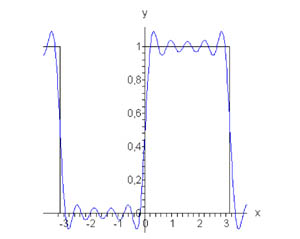
\includegraphics[height=.4\textwidth]{images/fourier_series_square.jpg}
	\end{center}
  High frequencies are required in order to create sharp corners.  This applies in the most ideal sense to square and triangle waves.
}


\frame{{Dirichlet Conditions}
	Our series converges to $f(x)$ if it satisfies the following conditions:
  \begin{itemize}
  	\item Is periodic of period $2\pi$
  	\item Is single-valued between $-\pi$ and $\pi$
  	\item Has finite number of max and min values
  	\item $\int_{-\pi}^\pi \lvert f(x)\rvert~dx$ is finite
  \end{itemize}
  We often do not  need to evaluate the integral if we can show that $f(x)$ is bounded.
}


\frame{{Complex Form of Fourier Series}
  We can use what we know about the complex representation of sines and cosines to rewrite the Fourrier series.
  \begin{block}{Complex Representation of Fourrier Series}
  	\begin{align*}
  		f(x) &= c_0+c_1e^{ix}+c_{-1}e^{-ix}+c_{2}e^{2ix}+c_{-2}^{-2ix}+\cdots \\
  		&= \sum_{n=-\infty}^{\infty}c_nd^{inx}
  	\end{align*}
  \end{block}
  We calculate the coefficients, $c_n$, as follows,
  \begin{block}{Complex Representation of Fourrier Series}
  	\[
  		c_n = \frac{1}{2\pi}\int_{-\pi}^{\pi}f(x)e^{-inx}dx
  	\]
  \end{block}
}


\frame{{Other Intervals}
  We can easily re-write our interval as,
  \begin{block}{Fourrier Series Expansion}
    \begin{align*}
      f(x) &= \frac{a_0}{2}+a_1\cos\frac{\pi x}{l}+a_2\cos\frac{2\pi x}{l}+\cdots \\
      &\qquad + b_1\sin\frac{\pi x}{l}+b_2\sin\frac{2\pi x}{l}+\cdots \\
      &= \frac{a_0}{2}+\sum_1^\infty\left( a_n\cos\frac{n\pi x}{l}+b_n\sin\frac{n\pi x}{l} \right) \\
      &= \sum_{-\infty}^{\infty}c_ne^{in\pi x/l}
    \end{align*}
  \end{block}
}


\frame{{Other Intervals (continued)}
  And the new formulae for the Fourrier coefficients becomes,
  \begin{block}{Fourier Coefficients}
    \begin{align*}
      a_n &= \frac{1}{l}\int_{-l}^{l}f(x)\cos\frac{n\pi x}{l}dx \\
      b_n &= \frac{1}{l}\int_{-l}^{l}f(x)\sin\frac{n\pi x}{l}dx \\
      c_n &= \frac{1}{2l}\int_{-l}^{l}f(x)e^{-in\pi x/l}dx
    \end{align*}
  \end{block}
}


\frame{{Questions?}
	\begin{center}
		
\includegraphics[width=.7\textwidth]{images/fin.png}
	\end{center}
}

\end{document}
